\documentclass{article}
\usepackage{amsmath}
\usepackage{enumerate}
\usepackage{fancyhdr} % Required for custom headers
\usepackage{lastpage} % Required to determine the last page for the footer
\usepackage{extramarks} % Required for headers and footers
\usepackage[usenames,dvipsnames]{color} % Required for custom colors
\usepackage{graphicx} % Required to insert images
\usepackage[tight,footnotesize]{subfigure} % Required for subfig
\usepackage{caption} % Required for subfig
\usepackage{hyperref} % Required for url
\usepackage{listings} % Required for insertion of code
\usepackage{courier} % Required for the courier font
\usepackage{lipsum} % Used for inserting dummy 'Lorem ipsum' text into the template
\topmargin=-0.45in
\evensidemargin=0in
\oddsidemargin=0in
\textwidth=6.5in
\textheight=9.0in
\headsep=0.25in
\linespread{1.1} % Line spacing
\pagestyle{fancy}
\lhead{\hmwkAuthorName} % Top left header
% \chead{\hmwkClass\ (\hmwkClassInstructor\ \hmwkClassTime): \hmwkTitle} % Top center head
\chead{\hmwkClass\ : \hmwkTitle} % Top center head
\rhead{\firstxmark} % Top right header
\lfoot{\lastxmark} % Bottom left footer
\cfoot{} % Bottom center footer
\rfoot{Page\ \thepage\ of\ \protect\pageref{LastPage}} % Bottom right footer
\renewcommand\headrulewidth{0.4pt} % Size of the header rule
\renewcommand\footrulewidth{0.4pt} % Size of the footer rule
\setlength\parindent{0pt} % Removes all indentation from paragraphs

% Define floor and ceiling
\def\lc{\left\lceil}   
\def\rc{\right\rceil}
\def\lf{\left\lfloor}   
\def\rf{\right\rfloor}

% Set your language 
%\lstset{language=Java}
\definecolor{codegreen}{rgb}{0,0.6,0}
\definecolor{codegray}{rgb}{0.5,0.5,0.5}
\definecolor{codepurple}{rgb}{0.58,0,0.82}
\definecolor{backcolour}{rgb}{0.95,0.95,0.92}
 
\lstdefinestyle{mystyle}{
    backgroundcolor=\color{backcolour},   
    commentstyle=\color{codegreen},
    keywordstyle=\color{magenta},
    numberstyle=\tiny\color{codegray},
    stringstyle=\color{codepurple},
    basicstyle=\footnotesize,
    breakatwhitespace=false,         
    breaklines=true,                 
    captionpos=b,                    
    keepspaces=true,                 
    numbers=left,                    
    numbersep=8pt,                  
    showspaces=false,                
    showstringspaces=false,
    showtabs=false,                  
    tabsize=2
}
\lstset{style=mystyle}

% Header and footer for when a page split occurs within a problem environment
\newcommand{\enterProblemHeader}[1]{
\nobreak\extramarks{#1}{#1 continued on next page\ldots}\nobreak
\nobreak\extramarks{#1 (continued)}{#1 continued on next page\ldots}\nobreak
}

% Header and footer for when a page split occurs between problem environments
\newcommand{\exitProblemHeader}[1]{
\nobreak\extramarks{#1 (continued)}{#1 continued on next page\ldots}\nobreak
\nobreak\extramarks{#1}{}\nobreak
}

\setcounter{secnumdepth}{0} % Removes default section numbers
\newcounter{homeworkProblemCounter} % Creates a counter to keep track of the number of problems

\newcommand{\homeworkProblemName}{}
\newenvironment{homeworkProblem}[1][Problem \arabic{homeworkProblemCounter}]{ % Makes a new environment called homeworkProblem which takes 1 argument (custom name) but the default is "Problem #"
\stepcounter{homeworkProblemCounter} % Increase counter for number of problems
\renewcommand{\homeworkProblemName}{#1} % Assign \homeworkProblemName the name of the problem
\section{\homeworkProblemName} % Make a section in the document with the custom problem count
\enterProblemHeader{\homeworkProblemName} % Header and footer within the environment
}{
\exitProblemHeader{\homeworkProblemName} % Header and footer after the environment
}

\newcommand{\problemAnswer}[1]{ % Defines the problem answer command with the content as the only argument
\noindent\framebox[\columnwidth][c]{\begin{minipage}{0.98\columnwidth}#1\end{minipage}} % Makes the box around the problem answer and puts the content inside
}

\newcommand{\homeworkSectionName}{}
\newenvironment{homeworkSection}[1]{ % New environment for sections within homework problems, takes 1 argument - the name of the section
\renewcommand{\homeworkSectionName}{#1} % Assign \homeworkSectionName to the name of the section from the environment argument
\subsection{\homeworkSectionName} % Make a subsection with the custom name of the subsection
\enterProblemHeader{\homeworkProblemName\ [\homeworkSectionName]} % Header and footer within the environment
}{
\enterProblemHeader{\homeworkProblemName} % Header and footer after the environment
}

\newlength{\tabcont}

\newcommand{\tab}[1]{%
\settowidth{\tabcont}{#1}%
\ifthenelse{\lengthtest{\tabcont < .25\linewidth}}%
{\makebox[.25\linewidth][l]{#1}\ignorespaces}%
{\makebox[.5\linewidth][l]{\color{red} #1}\ignorespaces}%
}%
%----------------------------------------------------------------------------------------
%	NAME AND CLASS SECTION
%----------------------------------------------------------------------------------------

\newcommand{\hmwkTitle}{Homework\ \#5} % Assignment title
\newcommand{\hmwkDueDate}{Monday,\ January\ 1,\ 2012} % Due date
\newcommand{\hmwkClass}{Fundamental Algorithms} % Course/class
\newcommand{\hmwkClassTime}{} % Class/lecture time
\newcommand{\hmwkClassInstructor}{Prof. Joel Spencer} % Teacher/lecturer
\newcommand{\hmwkAuthorName}{Songxiao Zhang, N10224459, {\tt 72}} % Your name

%----------------------------------------------------------------------------------------
%	TITLE PAGE
%----------------------------------------------------------------------------------------

\title{
\textmd{\textbf{\hmwkClass:\ \hmwkTitle}}\\
}
\author{\textbf{\hmwkAuthorName}}

\begin{document}

\maketitle

%----------------------------------------------------------------------------------------
%	PROBLEM 1
%----------------------------------------------------------------------------------------
\begin{homeworkProblem}
\begin{enumerate}[(a)]
    \item Since {\tt MERGE-SORT} takes $\Theta(nlgn)$. For $n^2$ items. 
          $$\Theta(n^2lg(n^2)) = \Theta(2n^2lgn) = \Theta(n^2lgn)$$
          
    \item $m=log_2n$, $\Theta(m^22^m) = \Theta(lg^2n \times 2^{log_2n}) = \Theta(nlg^2n)$
          
    \item $m=log_2n$, $\Theta(5^m) = \Theta(5^{log_2n}) = \Theta(n^{log_25})$
          
    \item {\tt COUNTING-SORT} takes $\Theta(n + k)$ where $k$ is the data range. To sort 
          $n^2$ items with each item in the range $0$ to $n^3-1$ takes
          $$\Theta(n^2 + n^3) = \Theta(n^3)$$
          
    \item {\tt RADIX-SORT} takes $\Theta(d(n+k))$ where $d$ is the number of digits and 
          $k$ is the data range for each digit. To sort $n^2$ items with each item in the 
          range $0$ to $n^3-1$ and base $n$ is used. \\ 
          $d=log_nn^3=3$ and $k=n$ $\Theta(d(n+k))=\Theta(3(n^2+n))=\Theta(n^2)$
\end{enumerate}
\end{homeworkProblem}

%----------------------------------------------------------------------------------------
%	PROBLEM 2
%----------------------------------------------------------------------------------------
\begin{homeworkProblem}
We can refer to this table (ASCII table - 64). 
\begin{lstlisting}[frame=single]
A  1	B  2	C  3	D  4	E  5	F  6	G  7	H  8	I  9	J  10	K  11	L  12	M  13
N  14	O  15	P  16	Q  17	R  18	S  19	T  20	U  21	V  22	W  23	X  24	Y  25	Z  26
\end{lstlisting}

COBB	 =22,	$22\%7=1$\\
RUTH	 =67,	$67\%7=4$\\
ROSE	 =57,	$57\%7=1$\\
BUZ	 =49,	$49\%7=0$\\
DOC	 =22,	$22\%7=1$\\
COBB	 =22,	$22\%7=1$\\

Insert COBB \quad
0:NULL, 1:COBB, 2:NULL, 3:NULL, 4:NULL, 5:NULL, 6:NULL

Insert RUTH \quad
0:NULL, 1:COBB, 2:NULL, 3:NULL, 4:RUTH, 5:NULL, 6:NULL

Insert ROSE \quad
0:NULL, 1:ROSE $\rightarrow$ COBB, 2:NULL, 3:NULL, 4:RUTH, 5:NULL, 6:NULL

Search BUZ  \quad   Return NULL at index 0.

Insert DOC  \quad
0:NULL, 1:DOC $\rightarrow$ ROSE $\rightarrow$ COBB, 2:NULL, 3:NULL, 4:RUTH, 5:NULL, 6:NULL

Delete COBB \quad
0:NULL, 1:DOC $\rightarrow$ ROSE, 2:NULL, 3:NULL, 4:RUTH, 5:NULL, 6:NULL
\end{homeworkProblem}

%----------------------------------------------------------------------------------------
%	PROBLEM 3
%----------------------------------------------------------------------------------------
\begin{homeworkProblem}
Assume the implementation of the hashtable is an array, each cell contains null if empty, or an pointer to the address of the head linked list for multiple elements in collision (with the same key). The base of hash function is the same as the size of the hashtable.  \\

By chaining, each cell only contains an address (4 bytes for 32-bit,  8 bytes for 64-bit host), incomparable to an record (10K byte). 1 million addresses takes $8 \times 10^6 = 8GB$ about 800 records. It's small ($4\%$) compare to 20000 records. \\

As the base of hash function is the same as the size of the hashtable, a larger hashtable can reduce hash collisions and therefore running time. During collision, {\tt SEARCH(item)} costs $\Theta(N)$ while it should be $\Theta(1)$.
\end{homeworkProblem}

%----------------------------------------------------------------------------------------
%	PROBLEM 4
%----------------------------------------------------------------------------------------
\begin{homeworkProblem}
% [a:80 [h:70] [d:200 [e:150 [c:140 [] [g:148 [f:143] [] ] ] [b:170] ] [] ]]
% [a:80 [h:70 [Null] [Null]] [d:200 [e:150 [c:140 [Null] [g:148 [f:143  [Null] [Null] ] [Null] ] ] [b:170 [Null] [Null]] ] [Null] ]]
% [a:80 [h:70 [Null] [Null]] [d:200 [e:150 [c:140 [i:100 [Null] [Null]] [g:148 [f:143  [Null] [Null] ] [Null] ] ] [b:170 [Null] [Null]] ] [Null] ]]
% http://mshang.ca/syntree/?i=[NP%20[N%20Alice]%20and%20[N%20Bob]]
The sequence I did is similar to breath-first search for the tree. 
    \begin{figure}[h]
        \centering
        \subfigure[]{\label{}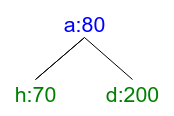
\includegraphics[scale=0.4]{hw5/1.png}}
        \subfigure[]{\label{}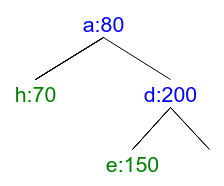
\includegraphics[scale=0.4]{hw5/2.png}}
        \subfigure[]{\label{}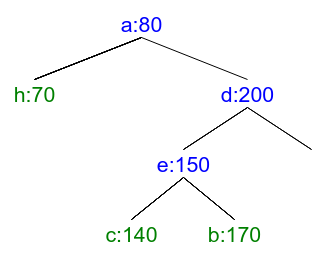
\includegraphics[scale=0.4]{hw5/3.png}}
        \subfigure[]{\label{}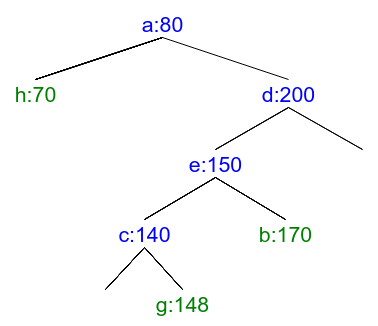
\includegraphics[scale=0.4]{hw5/4.png}}
        \subfigure[]{\label{}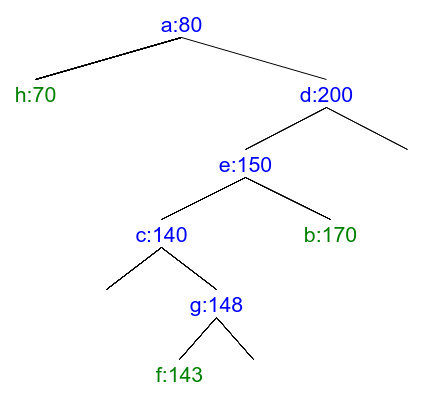
\includegraphics[scale=0.4]{hw5/5.png}}
        % \subfigure[]{\label{}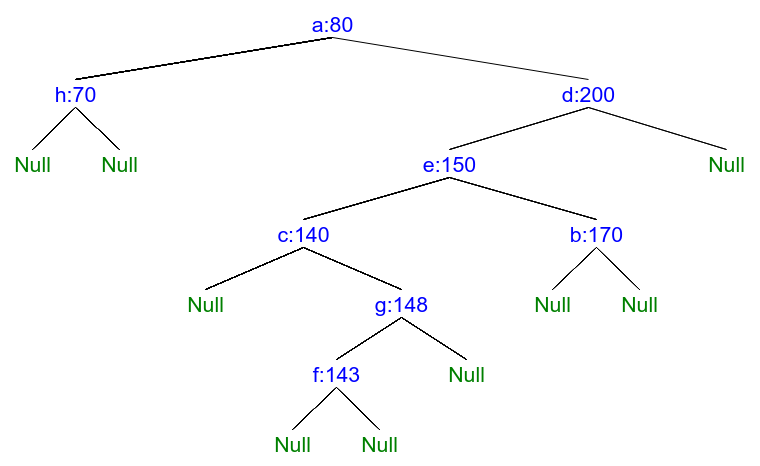
\includegraphics[scale=0.4]{hw5/6.png}}
        % \subfigure[]{\label{}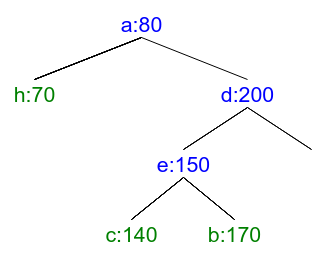
\includegraphics[width=0.45\textwidth]{hw5/3.png}}
        \caption{Each graph shows the result of 1 level like the breath-first search (the empty edges are required by the software drawing the graph)}
        \label{fig:flow}
    \end{figure} 
    
     \begin{figure}[h]
        \centering
        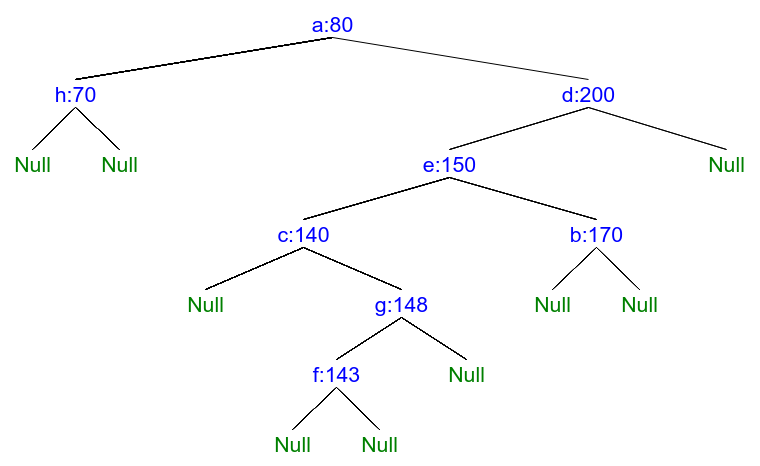
\includegraphics[scale=0.4]{hw5/6.png}
        \caption{The empty edges are required by the software drawing the graph. This is what it actually means. }
        \label{fig:flow}
    \end{figure}     \\~\\
    
    {\tt key[i]=100 $>$ key[a]=80} move to right d \\
    {\tt key[i]=100 $<$ key[d]=200} move to left e \\
    {\tt key[i]=100 $<$ key[e]=150} move to left c \\
    {\tt key[i]=100 $<$ key[c]=240} move to left Null \\
    c.left = Null, insert i here. 
    \begin{figure}[h!]
        \centering
        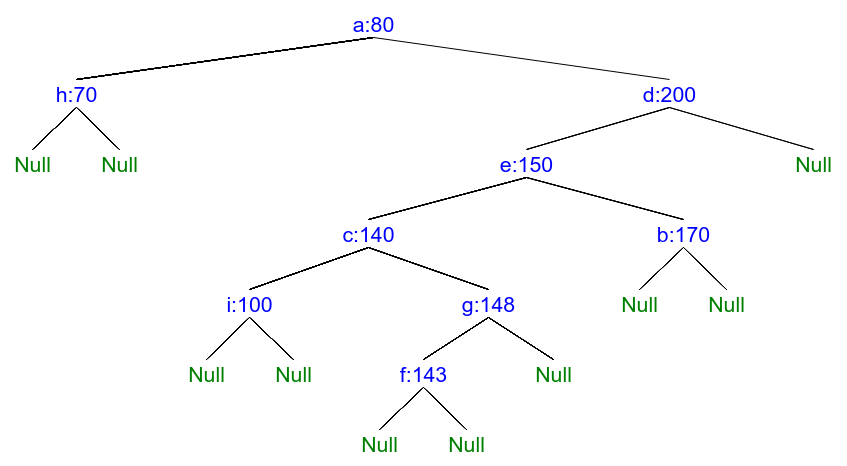
\includegraphics[scale=0.4]{hw5/7.png}
        \caption{}
        \label{fig:flow}
    \end{figure} 
    

% \begin{enumerate}[a.]
    % \item $T(n) = n^2+(n+1)^2+\ldots + (2n)^2 
    %       = \sum\limits_{i=0}^{2n} i^2 - \sum\limits_{i=0}^{n-1} i^2$, since
    %       $\sum\limits_{i=0}^{n} i^2 = \frac{n(n+1)(2n+1)}{6}$. 
    %       $$T(n) = \frac{2n(2n+1)(4n+1)}{6} - \frac{(n-1)(n-1+1)(2n-2+1)}{6} = \frac{14n^3+15n^2-n}{6}$$
    %       $g(n) = \Theta(n^3), c_1 = 2, c_2 = 3 $. 
    % \item $T(n) = \lg^2(1)+\lg^2(2)+\ldots + \lg^2(n) = \sum\limits_{i=0}^{n} lg^2 i $. 
    %       Approach from right $T(n) \leq nlg^2 n$, and approach from left by deleting first $n/2$ itmes
    %       $T(n) > (n/2) * lg^2(n/2)$ but $\frac{1}{2}$ can never get, we can take $\frac{1}{4}$ as a smaller number that we can reach. So we can get $g(n) = \Theta(nlg^2n), c_1 = 1/4, c_2 = 1 $. 
    % \item $T(n)=1^3+\ldots+n^3=\sum\limits_{i=1}^{n} \frac{n^2 \times (n+1)^2}{4} = \frac{n^4+2n^3+n^2}{4}$
    %       so $g(n) = \Theta(n^4), c_1 = 1/4, c_2 = 1 $
% \end{enumerate}
\end{homeworkProblem}


% \begin{lstlisting}[frame=single]
% \end{lstlisting}

% \begin{enumerate}[a.]
%     \item 
        %   
        %   
% \end{enumerate}
\end{document}